Tabular data, including product descriptions and features, is a major component of e-commerce, although natural language is used for most user interactions, such as Q\&A and helper agents. The need for models that can efficiently interpret tabular data and engage consumers through logical, context-aware communication is thus urgent.
\\\\
In order to meet this need, table-to-text creation is essential, particularly in e-commerce, where it makes it possible to provide user-specific summaries, customized descriptions, and product reviews. The ability to convert structured patient records into succinct summaries for physicians \cite{he2023survey} and turn tabular financial data into analytical reports \cite{Varshney_2024} are two examples of industries that possess this capability in addition to e-commerce. Despite its benefits, creating text that is both comprehensible and appropriate for the context from structured data is still quite difficult, especially when coordinating input data and goal outputs with user-specific needs.
\\\\
User or query-centric scenarios, which require high-quality datasets that capture domain-specific perspectives, exacerbate these difficulties. The depth needed for specialized applications such as product reviews is typically absent in existing table-to-text datasets, which tend to concentrate on general-purpose summaries \cite{macková2023promapdatasetsproductmapping}. The utility of datasets such as QTSUMM \cite{zhao2023qtsummqueryfocusedsummarizationtabular} for attribute-specific product reviews is limited because they provide tabular summaries that are unrelated to the product domain. Product-specific text production, on the other hand, needs to take into account a variety of characteristics (such as battery life and display quality) and adjust to different user intents, including offering technical details or condensed pros and drawbacks.
 
\begin{figure}[t]
    \centering
    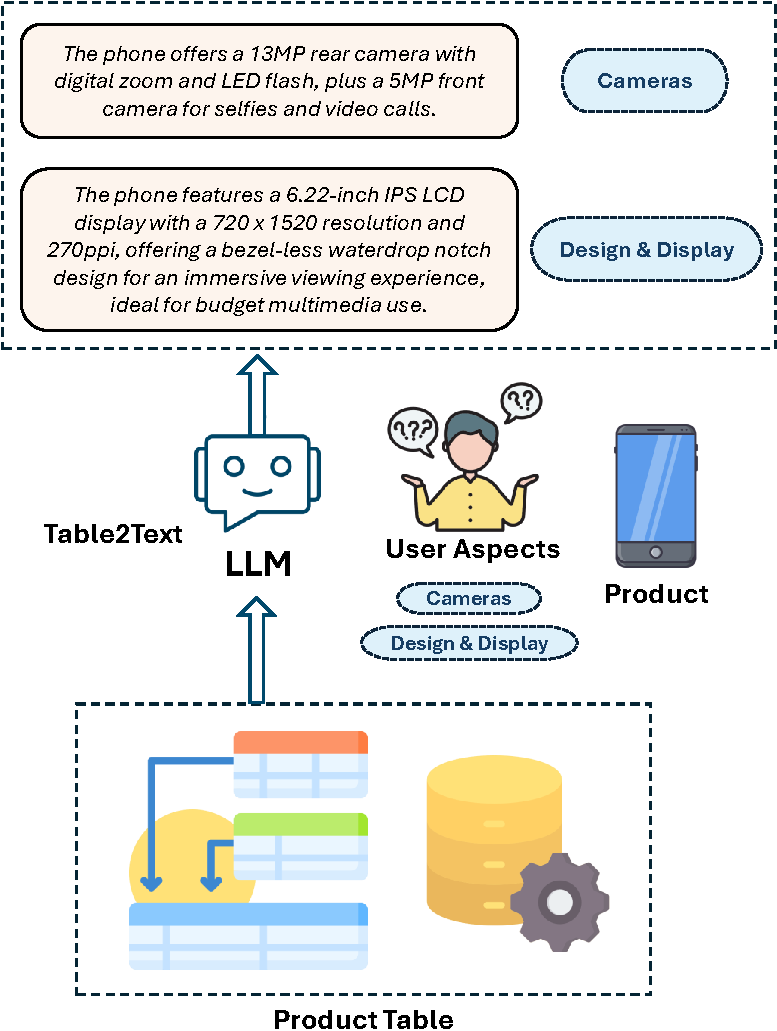
\includegraphics[scale = 0.60]{images/task-def.pdf}
    \caption{Product Table2Text}
    \label{fig:task-def}
\end{figure}

Problems with table-to-text creation have been addressed in previous publications. LLama2-chat \cite{jiang2023mistral} and StructLM \cite{gao2024jsontuning} are examples of fine-tuned models that have enhanced performance on table-based datasets by utilizing domain-specific training, while Large Language Models (LLMs) such as GPT-4 and BERT have specifically shown strong general-purpose text generation capabilities \cite{touvron2023llama, zhuang2024structlm}. To properly capture the subtleties of attribute-specific text creation for intricate e-commerce jobs, customized datasets are necessary, as existing methods are unable to handle the complexities of product-specific domains.

Table-to-text generation has benefited from datasets that provide structured data and annotated summaries, such as ROTOWIRE \cite{wiseman2017challengesdatatodocumentgeneration}, TabFact \cite{2019TabFactA}, and WikiTableT \cite{chen2021wikitabletlargescaledatatotextdataset}.  ROTOWIRE creates sports summaries, TabFact facilitates fact-checking, and WikiTableT concentrates on creating descriptions from Wikipedia tables. Nevertheless, the depth required for product-specific text generation is absent from these datasets. Although datasets like ToTTo \cite{parikh2020tottocontrolledtabletotextgeneration} and LogicNLG \cite{chen2020logicalnaturallanguagegeneration} emphasize logical deductions and sophisticated sentence extraction, their relevance to e-commerce is still restricted. The increasing demand for domain-specific datasets customized for product evaluations and attribute-specific summaries is highlighted by recent work \cite{He2023ReviewOS}.

This paper introduces a table-to-text dataset for the products domain and explores whether fine-tuned LLMs can bridge the gap between general-purpose capabilities and domain-specific needs in e-commerce. By leveraging tailored datasets and fine-tuning techniques, this work seeks to empower e-commerce platforms to generate more precise and engaging product reviews, enhancing customer satisfaction and business outcomes.
